\documentclass[a4paper]{article}
\usepackage{times}
\usepackage[utf8]{inputenc}
\usepackage{selinput}
\usepackage{upquote}
\usepackage[margin=2cm, rmargin=4cm, tmargin=3cm]{geometry}
\usepackage{tcolorbox}
\usepackage{xspace}
\usepackage[french]{babel}
\usepackage{url}
\usepackage{hyperref}
\usepackage{fontawesome5}
\usepackage{marginnote}
\usepackage{ulem}
\usepackage{tcolorbox}
\usepackage{graphicx}
%\usepackage[top=Bcm, bottom=Hcm, outer=Ccm, inner=Acm, heightrounded, marginparwidth=Ecm, marginparsep=Dcm]{geometry}


\newtcolorbox{Example}[1]{colback=white,left=20pt,colframe=slideblue,fonttitle=\bfseries,title=#1}
\newtcolorbox{Solutions}[1]{colback=white,left=20pt,colframe=green,fonttitle=\bfseries,title=#1}
\newtcolorbox{Conseils}[1]{colback=white,left=20pt,colframe=slideblue,fonttitle=\bfseries,title=#1}
\newtcolorbox{Warning}[1]{colback=white,left=20pt,colframe=warning,fonttitle=\bfseries,title=#1}

\setlength\parindent{0pt}

  %Exercice environment
  \newcounter{exercice}
  \newenvironment{Exercice}[1][]
  {
  \par
  \stepcounter{exercice}\textbf{Question \arabic{exercice}:} (\faClock \enskip \textit{#1})
  }
  {\bigskip}
  

% Title
\newcommand{\titre}{\begin{center}
  \section*{Algorithmes et Pensée Computationnelle}
\end{center}}
\newcommand{\cours}[1]
{\begin{center} 
  \textit{#1}\\
\end{center}
  }


\newcommand{\exemple}[1]{\newline~\textbf{Exemple :} #1}
%\newcommand{\attention}[1]{\newline\faExclamationTriangle~\textbf{Attention :} #1}

% Documentation url (escape \# in the TP document)
\newcommand{\documentation}[1]{\faBookOpen~Documentation : \href{#1}{#1}}

% Clef API
\newcommand{\apikey}[1]{\faKey~Clé API : \lstinline{#1}}
\newcommand{\apiendpoint}[1]{\faGlobe~Url de base de l'API \href{#1}{#1}}

%Listing Python style
\usepackage{color}
\definecolor{slideblue}{RGB}{33,131,189}
\definecolor{green}{RGB}{0,190,100}
\definecolor{blue}{RGB}{121,142,213}
\definecolor{grey}{RGB}{120,120,120}
\definecolor{warning}{RGB}{235,186,1}

\usepackage{listings}
\lstdefinelanguage{texte}{
    keywordstyle=\color{black},
    numbers=none,
    frame=none,
    literate=
           {é}{{\'e}}1
           {è}{{\`e}}1
           {ê}{{\^e}}1
           {à}{{\`a}}1
           {â}{{\^a}}1
           {ù}{{\`u}}1
           {ü}{{\"u}}1
           {î}{{\^i}}1
           {ï}{{\"i}}1
           {ë}{{\"e}}1
           {Ç}{{\,C}}1
           {ç}{{\,c}}1,
    columns=fullflexible,keepspaces,
	breaklines=true,
	breakatwhitespace=true,
}
\lstset{
    language=Python,
	basicstyle=\bfseries\footnotesize,
	breaklines=true,
	breakatwhitespace=true,
	commentstyle=\color{grey},
	stringstyle=\color{slideblue},
  keywordstyle=\color{slideblue},
	morekeywords={with, as, True, False, Float, join, None, main, argparse, self, sort, __eq__, __add__, __ne__, __radd__, __del__, __ge__, __gt__, split, os, endswith, is_file, scandir, @classmethod},
	deletekeywords={id},
	showspaces=false,
	showstringspaces=false,
	columns=fullflexible,keepspaces,
	literate=
           {é}{{\'e}}1
           {è}{{\`e}}1
           {ê}{{\^e}}1
           {à}{{\`a}}1
           {â}{{\^a}}1
           {ù}{{\`u}}1
           {ü}{{\"u}}1
           {î}{{\^i}}1
           {ï}{{\"i}}1
           {ë}{{\"e}}1
           {Ç}{{\,C}}1
           {ç}{{\,c}}1,
    numbers=left,
}

\newtcbox{\mybox}{nobeforeafter,colframe=white,colback=slideblue,boxrule=0.5pt,arc=1.5pt, boxsep=0pt,left=2pt,right=2pt,top=2pt,bottom=2pt,tcbox raise base}
\newcommand{\projet}{\mybox{\textcolor{white}{\small projet}}\xspace}
\newcommand{\optionnel}{\mybox{\textcolor{white}{\small Optionnel}}\xspace}
\newcommand{\advanced}{\mybox{\textcolor{white}{\small Pour aller plus loin}}\xspace}
\newcommand{\auto}{\mybox{\textcolor{white}{\small Auto-évaluation}}\xspace}


\usepackage{environ}
\newif\ifShowSolution
\NewEnviron{solution}{
  \ifShowSolution
	\begin{Solutions}{\faTerminal \enskip Solution}
		\BODY
	\end{Solutions}
  \fi}


  \usepackage{environ}
  \newif\ifShowConseil
  \NewEnviron{conseil}{
    \ifShowConseil
    \begin{Conseils}{\faLightbulb \quad Conseil}
      \BODY
    \end{Conseils}

    \fi}

    \usepackage{environ}
  \newif\ifShowWarning
  \NewEnviron{attention}{
    \ifShowWarning
    \begin{Warning}{\faExclamationTriangle \quad Attention}
      \BODY
    \end{Warning}

    \fi}
  

%\newcommand{\Conseil}[1]{\ifShowIndice\ \newline\faLightbulb[regular]~#1\fi}



\usepackage{array}
\newcolumntype{C}[1]{>{\centering\let\newline\\\arraybackslash\hspace{0pt}}m{#1}}

\begin{document}

% Change the following values to true to show the solutions or/and the hints
\ShowSolutiontrue
\ShowConseiltrue
\titre
\cours{Architecture des ordinateurs}

Le but de cette séance est de comprendre le fonctionnement d'un ordinateur. La série d'exercices sera axée autour de la conversion en base binaire, décimale ou hexadécimal d'une part et du modèle Von Neumann d'autre part. \\

\section{Conversions}

\begin{Exercice}[5 minutes]  \textbf{Conversion $Base_{10}$ - $Base_2$}\\
    \begin{enumerate}
        \item Convertir le nombre 10$_{(10)}$ en base 2.
        \item Convertir le nombre 45$_{(10)}$ en base 2.
        \item Convertir le nombre 173$_{(10)}$ en base 2.
    \end{enumerate}

    \begin{conseil}
    
        Vous pouvez utiliser la table des puissances de 2 pour vous aider. \\
        
        \begin{tabular}{| C{0.1\textwidth} | C{0.1\textwidth} | C{0.1\textwidth} | C{0.1\textwidth} | C{0.1\textwidth} | C{0.1\textwidth} | C{0.1\textwidth} |} 
            \hline
            \textbf{puissance} & $2^{5}$ & $2^{4}$ & $2^{3}$ & $2^{2}$ & $2^{1}$ & $2^{0}$ \\ [0.5ex] 
            \hline
            \textbf{valeur} & 32 & 16 & 8 & 4 & 2 & 1 \\ [0.5ex] 
            \hline
        \end{tabular} \\
        
        %Useful link: http://www.circuits-logiques.polymtl.ca/help/Chapitre05.pdf
    \end{conseil}
    \begin{solution}
        Il existe 2 méthodes pour simplifier la conversion d'un nombre de la base 10 à la base 2. Ici le nombre 45 sera entièrement développé. \\
        
        
        \textbf{Méthode 1 :} \\
        
        
        Prenez votre nombre et divisez le par 2 en colonne. S'il y a un reste, notez le à coté, sinon notez 0. Répétez l'opération avec le résultat que vous venez d'obtenir, et ce jusqu'à arriver à 0. Pour lire votre nombre en binaire, prenez la suite de 0 et 1 correspondants aux différents restes, mais prenez les de bas en haut. \\
       	
        \begin{tabular}{| C{0.1\textwidth} | C{0.1\textwidth} |} 
            \hline
            \textbf{nombre} & \textbf{reste}\\ [0.5ex]
            \hline
            173 &  - \\ [0.5ex] 
            \hline
            86 & 1 \\ [0.5ex] 
            \hline
            43 & 0 \\ [0.5ex] 
            \hline
            21 & 1 \\ [0.5ex] 
            \hline
            10 & 1 \\ [0.5ex] 
            \hline
            5 & 0 \\ [0.5ex] 
            \hline
            2 & 1 \\ [0.5ex] 
            \hline
	        1 & 0 \\ [0.5ex] 
            \hline
	        0 & 1 \\ [0.5ex] 
            \hline
            
        \end{tabular} \\

        Ici, on obtient 10101101$_{(2)}$ \\
        
        \textbf{Méthode 2 :} \\
        
        Cette deuxième méthode consiste à utiliser la table des puissances de 2 que voici, ensuite on regarde la plus grande valeur de cette table qui peut être soustraite à notre nombre. Une fois trouvée, on la soustrait, on ajoute 1 sous la case correspondante et on répète l'opération avec le résultat obtenu. Répétez l'opération jusqu'à obtenir 0\\
        
Ici, 45 - 32 = 13, puis 13- 8 = 5, puis 5-4 = 1, puis 1-1 = 0 \\
        
   		\begin{tabular}{| C{0.1\textwidth} | C{0.1\textwidth} | C{0.1\textwidth} | C{0.1\textwidth} | C{0.1\textwidth} | C{0.1\textwidth} | C{0.1\textwidth} |} 
            \hline
            \textbf{puissance} & $2^{5}$ & $2^{4}$ & $2^{3}$ & $2^{2}$ & $2^{1}$ & $2^{0}$ \\ [0.5ex] 
            \hline
            \textbf{valeur} & 32 & 16 & 8 & 4 & 2 & 1 \\ [0.5ex] 
            \hline
            \textbf{binaire} & 1 & 0 & 1 & 1 & 0 & 1 \\ [0.5ex] 
            \hline
        \end{tabular} \\
        
        On obtient donc 101101$_{(2)}$ \\
        
        Les réponses sont les suivantes :
        \begin{enumerate}
        \item 10$_{(10)}$ = 1010$_{(2)}$
        \item 45$_{(10)}$ = 101101$_{(2)}$
        \item 173$_{(10)}$ = 10101101$_{(2)}$
        \end{enumerate}
    \end{solution}
\end{Exercice}


\begin{Exercice}[15 minutes]  \textbf{Conversion $Base_{10}$ - $Base_3$, $Base_8$, $Base_{16}$}\\
    \begin{enumerate}
        \item Convertir le nombre 40$_{(10)}$ en base 8.
        \item Convertir le nombre 52$_{(10)}$ en base 3.
        \item Convertir le nombre 254$_{(10)}$ en base 16.
    \end{enumerate}

    \begin{conseil}
        S'inspirer de la solution de la question précédente. \\
        
        N'oubliez pas qu'en hexadécimal, A vaut 10, B vaut 11, C vaut 12, D vaut 13, E vaut 14 et F vaut 15 ! \\
    \end{conseil}
    \begin{solution}
        Dans cette solution, la méthode 1 sera utilisée pour 52 en base 3, et la méthode 2  pour 254 en base 16. \\
        
        \textbf{Méthode 1 pour 52 (ici, nous sommes en base 3 donc on divise par 3) :} \\
       	
        \begin{tabular}{| C{0.1\textwidth} | C{0.1\textwidth} |} 
            \hline
            \textbf{nombre} & \textbf{reste}\\ [0.5ex]
            \hline
            52 &  - \\ [0.5ex] 
            \hline
            17 & 1 \\ [0.5ex] 
            \hline
            5 & 2 \\ [0.5ex] 
            \hline
            1 & 2 \\ [0.5ex] 
            \hline
            0 & 1 \\ [0.5ex] 
            \hline
        \end{tabular} \\

        Ici, on obtient 1221$_{(3)}$ \\
        
        \textbf{Méthode 2 pour 254 (ici, nous sommes en base 10)} \\
        
        Ici, il faut prendre en compte le nombre de fois qu'on peut multiplier le nombre par la valeur de la puissance. Ici on a 256 qui est trop grand, il faut donc partir sur 16. On voit qu'on peut aller jusqu'à 15*16 qui vaut 240. Donc on entre 15 sous la valeur 16 et on soustrait. 254-240 = 14. Il nous reste donc 14*1, on met alors 14 sous la valeur 1. \\
        
   		\begin{tabular}{| C{0.1\textwidth} | C{0.1\textwidth} | C{0.1\textwidth} | C{0.1\textwidth} | C{0.1\textwidth} |} 
            \hline
            \textbf{puissance} & $16^{2}$ & $16^{1}$ & $16^{0}$ \\ [0.5ex] 
            \hline
            \textbf{valeur} & 256 & 16 & 1 \\ [0.5ex] 
            \hline
            \textbf{hexa} & 0 & 15 & 14 \\ [0.5ex] 
            \hline
        \end{tabular} \\
        
        On obtient donc 15 14 (qui s'écrit FE$_{(16)}$)\\
        
        Les réponses sont les suivantes :
        \begin{enumerate}
        \item 40$_{(10)}$ = 50$_{(8)}$
        \item 52$_{(10)}$ = 1221$_{(3)}$
        \item 254$_{(10)}$ = FE$_{(16)}$
        \end{enumerate}
    \end{solution}
\end{Exercice}

\begin{Exercice}[15 minutes] \textbf{Conversion $Base_{3}$ - $Base_{16}$ en $Base_8$}
    \begin{enumerate}
        \item Convertir le nombre 10110$_{(2)}$ en base 10.
        \item Convertir le nombre 4321$_{(5)}$ en base 10.
        \item Convertir le nombre ABC$_{(16)}$ en base 10.
    \end{enumerate}
    \begin{conseil}
        % Ici utilisez les tables de puissances utilisées pour la méthode 2 (présentée dans la solution du premier exercice). \\
        
        N'oubliez pas qu'en hexadécimal, A vaut 10, B vaut 11, C vaut 12, D vaut 13, E vaut 14 et F vaut 15 ! \\
    \end{conseil}
    \begin{solution}
        Reprenons la table des puissances utilisée précédemment (exemple avec ABC$_{(16)}$) : \\
        
        Ici, A vaut 10, B vaut 11 et C vaut 12 \\
        
        \begin{tabular}{| C{0.1\textwidth} | C{0.1\textwidth} | C{0.1\textwidth} | C{0.1\textwidth} | C{0.1\textwidth} |} 
            \hline
            \textbf{puissance} & $16^{2}$ & $16^{1}$ & $16^{0}$ \\ [0.5ex] 
            \hline
            \textbf{valeur} & 256 & 16 & 1 \\ [0.5ex] 
            \hline
            \textbf{hexa} & 10 & 11 & 12 \\ [0.5ex] 
            \hline
        \end{tabular} \\
        
        Ici on obtient donc 10*256 + 11*16 + 12*1 = 2560 + 176 + 12 = 2748$_{(10)}$ \\
        
        \begin{enumerate}
        \item Convertir le nombre 10110$_{(2)}$  = 22$_{(10)}$
        \item Convertir le nombre 4321$_{(5)}$ = 586$_{(10)}$
        \item Convertir le nombre ABC$_{(16)}$ = 2748$_{(10)}$
        \end{enumerate}
    
    \end{solution}

\end{Exercice}
\newpage

\section{Arithmétique binaire}

\begin{Exercice}[15 minutes] \textbf{Addition de nombres binaires}
    \begin{enumerate}
        \item Additionner \lstinline{01010101}$_{(2)}$ et \lstinline{10101010}$_{(2)}$
        \item Additionner \lstinline{01011111}$_{(2)}$ et \lstinline{10000001}$_{(2)}$
        \item Additionner \lstinline{01110100}$_{(2)}$ et \lstinline{00011010}$_{(2)}$
    \end{enumerate}
    \begin{conseil}
\textbf{Table d'addition binaire:}\\
        \begin{tabular}{| C{0.1\textwidth} | C{0.1\textwidth} | C{0.1\textwidth} | C{0.1\textwidth} | C{0.1\textwidth} | C{0.1\textwidth} |} 
            \hline
            retenue & 1 & 0 & 0 & 0 & 0 \\ [0.5ex] 
            \hline
            a & 0 & 1 & 1 & 0 & 0 \\ [0.5ex] 
            \hline
            b & 0 & 1 & 0 & 1 & 0 \\ [0.5ex] 
            \hline
            a+b & 1 & 0 & 1 & 1 & 0 \\ [0.5ex] 
            \hline
        \end{tabular}
    \end{conseil}
    
    \begin{solution}
        Il faut utiliser la table d'addition. Pour commencer, entrez a et b, puis commencez à additionner chaque colonne. Si l' addition vaut 1, le résultat est 1 et la retenue est 0. Si l'addition vaut 2, le résultat est 0 et la retenue est 1. Si l'addition vaut 3, le résultat est 1 et la retenue est 1. N'oubliez pas d' additionner également la retenue à chaque colonne ! \\
        
Voici un exemple pour le deuxième point : \\

        \begin{tabular}{| p{1cm} | p{1cm} | p{1cm} | p{1cm} | p{1cm} | p{1cm} | p{1cm} | p{1cm} | p{1cm} |} 
            \hline
	    retenue & 0 & 0 & 1 & 1 & 1 & 1 & 1 & 0 \\ [0.5ex]
	    \hline
            a & 0 & 1 & 0 & 1 & 1 & 1 & 1 & 1 \\ [0.5ex] 
            \hline
            b & 1 & 0 & 0 & 0 & 0 & 0 & 0 & 1 \\ [0.5ex] 
            \hline
            a + b & 1 & 1 & 1 & 0 & 0 & 0 & 0 & 0 \\ [0.5ex]
            \hline
        \end{tabular} \\
        
        On obtient donc 11100000$_{(2)}$ \\
        
        \begin{enumerate}
        \item Additionner 01010101$_{(2)}$ + 10101010$_{(2)}$ = 11111111$_{(2)}$
        \item Additionner 01011111$_{(2)}$ + 10000001$_{(2)}$ = 11100000$_{(2)}$
        \item Additionner 01110100$_{(2)}$ + 00011010$_{(2)}$ = 10001110$_{(2)}$
    	\end{enumerate}
    \end{solution}
\end{Exercice}

\begin{Exercice}[15 minutes] \textbf{Soustraction de nombres binaires}\\
    Effectuer les opérations suivantes:

    \begin{enumerate}
        \item 01111111$_{(2)}$ - 01000000$_{(2)}$
        \item 10000000$_{(2)}$ - 00000001$_{(2)}$
        \item 10101010$_{(2)}$ - 01010101$_{(2)}$
    \end{enumerate}

    \begin{conseil}
        \textbf{Table de soustraction binaire:}\\
         \begin{tabular}{| C{0.1\textwidth} | C{0.1\textwidth} | C{0.1\textwidth} | C{0.1\textwidth} | C{0.1\textwidth} |} 
            \hline
            retenue & 0 & 1 & 0 & 0 \\ [0.5ex] 
            \hline
            a & 1 & 1 & 0 & 0 \\ [0.5ex] 
            \hline
            b & 1 & 0 & 1 & 0 \\ [0.5ex] 
            \hline
            a-b & 0 & 0 & 1 & 0 \\ [0.5ex] 
            \hline
        \end{tabular}
    \end{conseil}
    
    \begin{solution}
         Il faut utiliser la table de soustraction. Pour commencer, entrez a et b, puis commencez à soustraire chaque colonne. Si la soustraction vaut 0, le résultat est 0 et la retenue est 0. Si la soustraction vaut 1, le résultat est 1 et la retenue est 0. Si la soustraction vaut -1, le résultat est 1 et la retenue est 1. Si la soustraction vaut -2, le résultat est 0 et la retenue est 1. N'oubliez pas de soustraire la retenue à chaque fois ! \\

Voici un exemple pour le deuxième point : \\
 
\begin{tabular}{| p{1cm} | p{1cm} | p{1cm} | p{1cm} | p{1cm} | p{1cm} | p{1cm} | p{1cm} | p{1cm} |} 
            \hline
	    retenue & 0 & 1 & 1 & 1 & 1 & 1 & 1 & 0 \\ [0.5ex]
	    \hline
            a & 1 & 0 & 0 & 0 & 0 & 0 & 0 & 0 \\ [0.5ex] 
            \hline
            b & 0 & 0 & 0 & 0 & 0 & 0 & 0 & 1 \\ [0.5ex] 
            \hline
            a - b & 0 & 1 & 1 & 1 & 1 & 1 & 1 & 1 \\ [0.5ex]
            \hline
        \end{tabular} \\
 		
 		On obtient donc 1111111$_{(2)}$ \\
 		
 		\begin{enumerate}
        \item 01111111$_{(2)}$ - 01000000$_{(2)}$ = 111111$_{(2)}$
        \item 10000000$_{(2)}$ - 00000001$_{(2)}$ = 1111111$_{(2)}$
        \item 10101010$_{(2)}$ - 01010101$_{(2)}$ = 1010101$_{(2)}$
    \end{enumerate}
    \end{solution}

    \textbf{\\ \faTerminal  Exemple:}
        \begin{figure}[h]
            \centering
            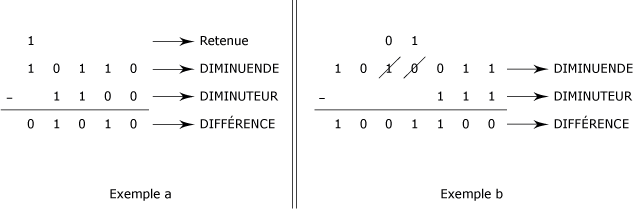
\includegraphics[width=0.52\textwidth]{img/substract.png}
            \caption{Exemple de soustraction de nombres binaires}
        \end{figure}

\end{Exercice}
\newpage

\section{Conversion et arithmétique}

\section{EXERCICES AVANCÉS - Conversion et arithmétique}

\begin{note}
    Ces exercices sont une une combinaison des parties 1 et 2 du TP. Ils ne sont donc pas absolument nécessaires à la compréhension du cours, mais \textbf{il est fortement recommandé de les faire.}\\
\end{note}

\begin{note}
    Ces deux exercices devraient être des exercices avancés\\
\end{note}


\begin{Exercice}[20 minutes] \textbf{Conversion et addition:}\\
    Effectuer les opérations suivantes:
    \begin{enumerate}
        \item 111101$_{(2)}$ + 110$_{(2)}$ = ...$_{(10)}$
        \item 111111$_{(2)}$ + 000001$_{(2)}$ = ...$_{(10)}$
        \item 127$_{(10)}$ + ABC$_{(16)}$ = ...$_{(10)}$
    \end{enumerate}
    \begin{conseil}
        Calculez à l'aide du tableau d'addition binaire ci-dessus ou une autre méthode que vous préférez.\\
        Additionnez les nombres lorsqu'ils sont dans la même base puis convertissez les dans la base souhaitée.\\
        
        Exemple de conversion : 1001000$_{(2)}$ = 72$_{(10)}$\\
        \addvbuffer[4pt 20pt]{\begin{tabular}{| C{0.15\textwidth} | C{0.07\textwidth} | C{0.07\textwidth} | C{0.07\textwidth} | C{0.07\textwidth} | C{0.07\textwidth} | C{0.07\textwidth} | C{0.07\textwidth} | C{0.06\textwidth} |} 
            \hline
            Base$_{(2)}$ & \textbf{1} & \textbf{0} & \textbf{0} & \textbf{1} & \textbf{0} & \textbf{0} & \textbf{0} & \textbf{}\\ [0.5ex]
            \hline
            Position$_{(2)}$ & $2^6$ & $2^5$ & $2^4$ & $2^3$ & $2^2$ & $2^1$ & $2^0$ & \\ [0.5ex] 
            \hline
             & $\downarrow$ & $\downarrow$ & $\downarrow$ & $\downarrow$ & $\downarrow$ & $\downarrow$ & $\downarrow$ & \\ [0.5ex] 
            \hline
            Équivalent$_{(10)}$ & 1 x $2^6$ & 0 x $2^5$ & 0 x $2^4$ & 1 x $2^3$ & 0 x $2^2$ & 0 x $2^1$ & 0 x $2^0$ & \\ [0.5ex]     
            \hline
            Valeurs$_{(10)}$ & 64 & 0 & 0 & 8 & 0 & 0 & 0 & = \textbf{72} \\ [0.5ex]
            \hline
        \end{tabular}}

        Rappel: Les valeurs en hexadécimale (base 16)\\
        \addvbuffer[4pt 20pt]{\begin{tabular}{| C{0.030\textwidth} | C{0.030\textwidth} | C{0.030\textwidth} | C{0.030\textwidth} | C{0.030\textwidth} | C{0.030\textwidth} | C{0.030\textwidth} | C{0.030\textwidth} | C{0.030\textwidth} | C{0.030\textwidth} | C{0.030\textwidth} | C{0.030\textwidth} | C{0.030\textwidth} | C{0.030\textwidth} | C{0.030\textwidth} | C{0.030\textwidth} |} 
            \hline
            \textbf{0} & \textbf{1} & \textbf{2} & \textbf{3} & \textbf{4} & \textbf{5} & \textbf{6} & \textbf{7} & \textbf{8} & \textbf{9} & \textbf{A} & \textbf{B} & \textbf{C} & \textbf{D} & \textbf{E} & \textbf{F}\\ [0.5ex]
            \hline
            0 & 1 & 2 & 3 & 4 & 5 & 6 & 7 & 8 & 9 & 10 & 11 & 12 & 13 & 14 & 15 \\ [0.5ex] 
            \hline
        \end{tabular}}

        Exemple de conversion : 3BF$_{(16)}$ = 959$_{(10)}$\\
        \addvbuffer[4pt 20pt]{\begin{tabular}{| C{0.15\textwidth} | C{0.15\textwidth} | C{0.15\textwidth} | C{0.15\textwidth} | C{0.1\textwidth} |} 
            \hline
            Base$_{(16)}$ & \textbf{3} & \textbf{B} & \textbf{F} & \textbf{}\\ [0.5ex]
            \hline
             Valeurs$_{(16)}$ & 3 & 11 & 15 & \\ [0.5ex]
             \hline
             Position$_{(16)}$ & $16^2$ & $16^1$ & $16^0$ & \\ [0.5ex] 
            \hline
             & $\downarrow$ & $\downarrow$ & $\downarrow$ & \\ [0.5ex] 
            \hline
            Équivalent$_{(10)}$ & 3 x $16^2$ & 11 x $16^1$ & 15 x $16^0$ &\\ [0.5ex]     
            \hline
            Valeurs$_{(10)}$ & 768 & 176 & 15 & = \textbf{959} \\ [0.5ex]
            \hline
        \end{tabular}}
        
        Exemple de conversion : 123$_{(10)}$ = ...$_{(8)}$\\
        
        $8^0 = 1 < 123$\qquad
        $8^1 = 8 < 123$\qquad
        $8^2 = 64 < 123$\qquad
        $8^3 = 512 > 123$\\
        
        $123 / 8 = 15$ avec un reste de \textbf{3}\\
        $15 / 8 = 1$ avec un reste de \textbf{7}\\
        $1 / 8 = 0$ avec un reste de \textbf{1}\\\
        
        \textbf{123$_{(10)}$ = 173$_{(8)}$}\\
        
    \end{conseil}
    \begin{solution} \textbf{6.1}\\
        Calcul du résultat en base 2:\\
        111101$_{(2)}$ + 110$_{(2)}$ = 1000011$_{(2)}$\\\\
        Conversion en base décimale:\\
        1000011$_{(2)}$ = 67$_{(10)}$\\\\
        Réponse :\\
        111101$_{(2)}$ + 110$_{(2)}$ = \textbf{67$_{(10)}$}\\
        
        \begin{tabular}{| C{0.15\textwidth} | C{0.07\textwidth} | C{0.07\textwidth} | C{0.07\textwidth} | C{0.07\textwidth} | C{0.07\textwidth} | C{0.07\textwidth} | C{0.07\textwidth} | C{0.06\textwidth} |} 
            \hline
            Base$_{(2)}$ & \textbf{1} & \textbf{0} & \textbf{0} & \textbf{0} & \textbf{0} & \textbf{1} & \textbf{1} & \textbf{}\\ [0.5ex]
            \hline
             & $2^6$ & $2^5$ & $2^4$ & $2^3$ & $2^2$ & $2^1$ & $2^0$ & \\ [0.5ex] 
            \hline
             & $\downarrow$ & $\downarrow$ & $\downarrow$ & $\downarrow$ & $\downarrow$ & $\downarrow$ & $\downarrow$ & \\ [0.5ex] 
            \hline
            Équivalent$_{(10)}$ & 1 x $2^6$ & 0 x $2^5$ & 0 x $2^4$ & 0 x $2^3$ & 0 x $2^2$ & 1 x $2^1$ & 1 x $2^0$ & \\ [0.5ex]     
            \hline
            Valeurs$_{(10)}$ & 64 & 0 & 0 & 0 & 0 & 2 & 1 & = 67 \\ [0.5ex]
            \hline
        \end{tabular}
        
    \end{solution}
    \begin{solution} \textbf{6.2}\\
        Calcul du résultat en base 2:\\
        111111$_{(2)}$ + 000001$_{(2)}$ = 1000000$_{(2)}$\\\\
        Conversion en base décimale:\\
        1000000$_{(2)}$ = 64$_{(10)}$\\\\
        Réponse :\\
        111111$_{(2)}$ + 000001$_{(2)}$ = \textbf{64$_{(10)}$}\\
    
        \textbf{6.3}\\
        ABC$_{(16)}$ = 2748$_{(10)}$ (Conversion en base 10)\\
       
        \addvbuffer[0pt 10pt]{\begin{tabular}{| C{0.15\textwidth} | C{0.08\textwidth} | C{0.08\textwidth} | C{0.08\textwidth} | C{0.08\textwidth} |} 
            \hline
            Base$_{(16)}$ & \textbf{A} & \textbf{B} & \textbf{C} & \textbf{}\\ [0.5ex]
            \hline
             & 10 & 11 & 12 & \\ [0.5ex]
             \hline
             & $16^2$ & $16^1$ & $16^0$ & \\ [0.5ex] 
            \hline
             & $\downarrow$ & $\downarrow$ & $\downarrow$ & \\ [0.5ex] 
            \hline
            Équivalent$_{(10)}$ & 10 x $16^2$ & 11 x $16^1$ & 12 x $16^0$ &\\ [0.5ex]     
            \hline
            Valeurs$_{(10)}$ & 2560 & 176 & 12 & = 2748 \\ [0.5ex]
            \hline
        \end{tabular}} 
        
        127$_{(10)}$ + 2748$_{(10)}$ = 2875$_{(10)}$ = 2875\\
        En commençant par zéro, augmentez 8 à des puissances entières de plus en plus grandes jusqu'à ce que le résultat dépasse 2875.\\
        
        \addvbuffer[0pt 10pt]{\begin{tabular}{| C{0.08\textwidth} | C{0.08\textwidth} | C{0.08\textwidth} | C{0.08\textwidth} | C{0.08\textwidth} | C{0.08\textwidth} |} 
            \hline
            Entier & 4 & 3 & 2 & 1 & 0\\ [0.5ex]
            \hline
             & $8^4$ & $8^3$ & $8^2$ & $8^1$ & $8^0$\\ [0.5ex]
            \hline
             & $\downarrow$ & $\downarrow$ & $\downarrow$ & $\downarrow$ & $\downarrow$\\ [0.5ex] 
            \hline
             Valeurs & 4096 & 512 & 64 & 8 & 1\\ [0.5ex] 
            \hline
        \end{tabular}}
        
        Déterminez les puissances de 8 qui seront utilisées pour placer les chiffres dans la représentation en base 8.\\

        $8^3$   $8^2$   $8^1$   $8^0$ \\

        Déterminez la valeur du premier chiffre en partant de la droite (correspondant à $8^0$) grâce au reste de la division entière.\\
        2875 / 8 = 359 avec un reste de \textbf{3}\\\\
        Divisez la partie numérique entière du quotient précédent, 359, par 8 et trouvez le reste. Le reste est le chiffre suivant (correspondant à $8^1$):\\
        359 / 8 = 44 avec un reste de \textbf{7}\\\\
        Ainsi de suite... la valeur pour $8^2$:\\
        44 / 8 = 5 avec un reste de \textbf{4}\\\\
        La valeur pour $8^3$:\\
        5 / 8 = 0 avec un reste de \textbf{5}\\

        2875$_{(10)}$ = \textbf{5473$_{(8)}$}    
    \end{solution} 

\end{Exercice}

\begin{Exercice}[20 minutes] \textbf{Conversion et soustraction:}\\
    Effectuer les opérations suivantes:
    \begin{enumerate}
        \item 101010$_{(2)}$ - 010101$_{(2)}$ = ...$_{(10)}$
        \item 64$_{(10)}$ - 001000$_{(2)}$ = ...$_{(10)}$
        \item FFF$_{(16)}$ - 127$_{(10)}$ = ...$_{(2)}$
    \end{enumerate}
    \begin{conseil}
            Si besoin, référez-vous aux éléments des conseils précédents.\\\ 
            
            Calculez à l'aide du tableau de soustraction binaire ci-dessus ou une autre méthode que vous préférez.\\\
            
            Additionnez les nombres lorsqu'ils sont dans la même base puis convertissez les dans la base souhaitée.\\\
            
            Exemple de conversion : 1001000$_{(2)}$ = 72$_{(10)}$\\
            \addvbuffer[4pt 20pt]{\begin{tabular}{| C{0.15\textwidth} | C{0.07\textwidth} | C{0.07\textwidth} | C{0.07\textwidth} | C{0.07\textwidth} | C{0.07\textwidth} | C{0.07\textwidth} | C{0.07\textwidth} | C{0.06\textwidth} |} 
            \hline
            Base$_{(2)}$ & \textbf{1} & \textbf{0} & \textbf{0} & \textbf{1} & \textbf{0} & \textbf{0} & \textbf{0} & \textbf{}\\ [0.5ex]
            \hline
            Position$_{(2)}$ & $2^6$ & $2^5$ & $2^4$ & $2^3$ & $2^2$ & $2^1$ & $2^0$ & \\ [0.5ex] 
            \hline
             & $\downarrow$ & $\downarrow$ & $\downarrow$ & $\downarrow$ & $\downarrow$ & $\downarrow$ & $\downarrow$ & \\ [0.5ex] 
            \hline
            Équivalent$_{(10)}$ & 1 x $2^6$ & 0 x $2^5$ & 0 x $2^4$ & 1 x $2^3$ & 0 x $2^2$ & 0 x $2^1$ & 0 x $2^0$ & \\ [0.5ex]     
            \hline
            Valeurs$_{(10)}$ & 64 & 0 & 0 & 8 & 0 & 0 & 0 & = \textbf{72} \\ [0.5ex]
            \hline
            \end{tabular}}
            
            
            Rappel: Les valeurs en hexadécimale (base 16)\\
            \begin{tabular}{| C{0.030\textwidth} | C{0.030\textwidth} | C{0.030\textwidth} | C{0.030\textwidth} | C{0.030\textwidth} | C{0.030\textwidth} | C{0.030\textwidth} | C{0.030\textwidth} | C{0.030\textwidth} | C{0.030\textwidth} | C{0.030\textwidth} | C{0.030\textwidth} | C{0.030\textwidth} | C{0.030\textwidth} | C{0.030\textwidth} | C{0.030\textwidth} |} 
            \hline
            \textbf{0} & \textbf{1} & \textbf{2} & \textbf{3} & \textbf{4} & \textbf{5} & \textbf{6} & \textbf{7} & \textbf{8} & \textbf{9} & \textbf{A} & \textbf{B} & \textbf{C} & \textbf{D} & \textbf{E} & \textbf{F}\\ [0.5ex]
            \hline
            0 & 1 & 2 & 3 & 4 & 5 & 6 & 7 & 8 & 9 & 10 & 11 & 12 & 13 & 14 & 15 \\ [0.5ex] 
            \hline
        \end{tabular}
        
        Exemple de conversion : 123$_{(10)}$ = ...$_{(2)}$\\
        
        $2^0 = 1 < 123$\qquad
        $2^1 = 2 < 123$\qquad
        $2^2 = 4 < 123$\qquad
        $2^3 = 8 < 123$\qquad
        $2^4 = 16 < 123$\qquad
        $2^5 = 32 < 123$\qquad
        $2^6 = 64 < 123$\qquad
        $2^7 = 128 > 123$\\
        
        $123 / 2 = 61$ avec un reste de \textbf{1} (premier chiffre en partant de droite)\\
        $61 / 2 = 30$ avec un reste de \textbf{1}\\
        $30 / 2 = 15$ avec un reste de \textbf{0}\\
        $15 / 2 = 7$ avec un reste de \textbf{1}\\
        $7 / 2 = 3$ avec un reste de \textbf{1}\\
        $3 / 2 = 1$ avec un reste de \textbf{1}\\
        $1 / 2 = 0$ avec un reste de \textbf{1} (dernier chiffre en partant de droite)\\\
        
        123$_{(10)}$ = \textbf{1111011$_{(2)}$}\\
        
        
    \end{conseil}
    \begin{solution} \textbf{7.1}\\
        Calcul du résultat en base 2:\\
        101010$_{(2)}$ - 010101$_{(2)}$ = 010101$_{(2)}$\\\\
        Conversion en base décimale:\\
        010101$_{(2)}$ = 21$_{(10)}$\\\\
        Réponse:\\
        101010$_{(2)}$ - 010101$_{(2)}$ = \textbf{21$_{(10)}$}\\
    \end{solution}
    
    \begin{solution} \textbf{7.2}\\
        Conversion de 001000$_{(2)}$ en base 10 :\\
        001000$_{(2)}$ = $2^3$ = 8$_{(10)}$\\
        
        Calcul du résultat en base 10:\\
        64$_{(10)}$ - 8$_{(10)}$ = 56$_{(10)}$\\\\
        
        Réponse : \\
        64$_{(10)}$ - 001000$_{(2)}$ = \textbf{56$_{(10)}$}

    \end{solution}
    
    \begin{solution} \textbf{7.3}\\
        Conversion de FFF$_{(16)}$ en base 10:\\
        FFF$_{(16)}$ = 4095$_{(10)}$\\\\
        Calcul en base décimale:\\
        4095$_{(10)}$ - 127$_{(10)}$ = 3968$_{(10)}$\\\\
        Convertir 3968$_{(10)}$ en base binaire :\\
        En commençant par zéro, augmentez 2 à des puissances entières de plus en plus grandes jusqu'à ce que le résultat dépasse 3968.\\
        Déterminez les puissances de 2 qui seront utilisées comme les places des chiffres dans la représentation en base 2 de 3968 :\\

        \addvbuffer[0pt 10pt]{\begin{tabular}{| C{0.06\textwidth} | C{0.06\textwidth} | C{0.06\textwidth} | C{0.04\textwidth} | C{0.04\textwidth} | C{0.04\textwidth} | C{0.035\textwidth} | C{0.035\textwidth} | C{0.035\textwidth} | C{0.035\textwidth} | C{0.035\textwidth} | C{0.035\textwidth} | C{0.035\textwidth} | C{0.035\textwidth} |} 
            \hline
             $2^{12}$ & $2^{11}$ & $2^{10}$ & $2^9$ & $2^8$ & $2^7$ & $2^6$ & $2^5$ & $2^4$ & $2^{3}$ & $2^2$ & $2^1$ & $2^0$\\ [0.5ex]
            \hline
            $\downarrow$ & $\downarrow$ & $\downarrow$ & $\downarrow$ & $\downarrow$ & $\downarrow$ & $\downarrow$ & $\downarrow$ & $\downarrow$ & $\downarrow$ & $\downarrow$ & $\downarrow$ & $\downarrow$\\ [0.5ex] 
            \hline
            4096 & 2048 & 1024 & 512 & 256 & 128 & 64 & 32 & 16 & 8 & 4 & 2 & 1\\ [0.5ex]
            \hline
        \end{tabular}}
        
        Déterminez la valeur du premier chiffre en partant de la droite (correspondant à $2^0$) grâce au reste de la division entière.\\
        3968 / 2 = 1984 avec un reste de \textbf{0}\\
        Divisez la partie numérique entière du quotient précédent, 1984, par 2 et trouvez le reste. Le reste est le chiffre suivant (correspondant à $2^1$):\\
        1984 / 2 = 992 avec un reste de \textbf{0}\\
        Ainsi de suite... Pour $2^2$\\
        992 / 2 = 496 avec un reste de \textbf{0}\\
        Pour $2^3$\\
        496 / 2 = 258 avec un reste de \textbf{0}\\
        Pour $2^4$\\
        258 / 2 = 124 avec un reste de \textbf{0}\\
        Pour $2^5$\\
        124 / 2 = 62 avec un reste de \textbf{0}\\
        Pour $2^6$\\
        62 / 2 = 31 avec un reste de \textbf{0}\\
        Pour $2^7$\\
        31 / 2 = 15 avec un reste de \textbf{1}\\
        Pour $2^8$\\
        15 / 2 = 7 avec un reste de \textbf{1}\\
        Pour $2^9$\\
        7 / 2 = 3 avec un reste de \textbf{1}\\
        Pour $2^10$\\
        3 / 2 = 1 avec un reste de \textbf{1}\\
        Pour $2^11$\\
        1 / 2 = 0 avec un reste de \textbf{1}\\\\

        3968$_{(10)}$ = 111110000000$_{(2)}$\\\\

        Réponse:\\
        FFF$_{(16)}$ - 127$_{(10)}$ = \textbf{111110000000$_{(2)}$}
    \end{solution}

\end{Exercice}


\newpage
\section{Modèle de Von Neumann}
Dans cette section, nous allons simuler une opération d'addition dans le \textbf{modèle de Van Neumann}, il va vous être demandé à chaque étape (FDES) de donner la valeur des registres.\\

\textbf{État d'origine:}\\
A l'origine, notre \lstinline{Program Counter (PC)} vaut \lstinline{00100000}.\\

Dans la mémoire, les instructions sont les suivantes:

\begin{tabular}{| C{0.1\textwidth} | C{0.1\textwidth} |} 
    \hline
    \textbf{Adresse} & \textbf{Valeur}\\ [0.5ex]
    \hline
    00011111 & 00100100\\ [0.5ex] 
    \hline
    00100000 & 10110110\\ [0.5ex] 
    \hline
    00100001 & 11101101\\ [0.5ex]
    \hline
\end{tabular}
\\\\
Les registres contiennent les valeurs suivantes:

\begin{tabular}{| C{0.1\textwidth} | C{0.1\textwidth} |} 
    \hline
    \textbf{Registre} & \textbf{Valeur}\\ [0.5ex]
    \hline
    00 & 11100011\\ [0.5ex] 
    \hline
    01 & 01101100\\ [0.5ex] 
    \hline
    10 & 00100101\\ [0.5ex] 
    \hline
    11 & 00000000\\ [0.5ex]
    \hline
\end{tabular}
\\\\
Les opérations disponibles pour l'unité de contrôle sont les suivantes:
\\
\begin{tabular}{| C{0.1\textwidth} | C{0.1\textwidth} |} 
    \hline
    \textbf{Numéro} & \textbf{Valeur}\\ [0.5ex]
    \hline
    00 & MOV\\ [0.5ex] 
    \hline
    01 & XOR\\ [0.5ex] 
    \hline
    10 & ADD\\ [0.5ex] 
    \hline
    11 & SUB\\ [0.5ex]
    \hline
\end{tabular}
\\\\


\begin{Exercice}[5 minutes]\textbf{Fetch}\\
    À la fin de l'opération \lstinline{FETCH}, quelles sont les valeurs du \lstinline{Program Counter} et de l'\lstinline{Instruction Register}?

    \begin{conseil}
        Pour rappel, l'\textbf{unité de contrôle (Control Unit)} commande et contrôle le fonctionnement du système. Elle est chargée du \textbf{séquençage} des opérations. Après chaque opération \lstinline{FETCH}, la valeur du \textbf{Program Counter} est incrémentée (valeur initiale + 1).
    \end{conseil}

    \begin{solution}
        À la fin de l'opération \lstinline{Fetch}, le \lstinline{Program Counter} vaudra \lstinline{00100001} tandis que l'\lstinline{Instruction Register} vaudra \lstinline{10110110}, ce qui correspond à la valeur de l'adresse mémoire \lstinline{00100000}.
    \end{solution}
\end{Exercice}

\begin{Exercice}[5 minutes] \textbf{Decode}
    \begin{enumerate}
        \item Quelle est la valeur de l'opération à exécuter?
        \item Quelle est l'adresse du registre dans lequel le résultat doit être enregistré?
        \item Quelle est la valeur du premier nombre de l'opération?
        \item Quelle est la valeur du deuxième nombre de l'opération?
    \end{enumerate}

    \begin{conseil}
        Pensez à décomposer la valeur de l'\lstinline{Instruction Register} pour obtenir toutes les informations demandées. \\
        Utilisez la même convention que celle présentée dans les diapositives du cours (Computer Architecture - Page 15) \\
        Les données issues de la décomposition de l'\lstinline{Instruction Register} ne sont pas des valeurs brutes, mais des références. Trouvez les tables concordantes pour y récupérer les valeurs.
    \end{conseil}

    \begin{solution}
        En décomposant l'\lstinline{Instruction Register} (10110110), on obtient les données suivantes:
        \begin{itemize}
            \item \lstinline{10}, correspond à l'opération à effectuer,
            \item \lstinline{11}, correspond à \textbf{l'adresse} du registre où sera sauvegardé le résultat,
            \item \lstinline{01}, correspond à \textbf{l'adresse} du premier nombre,
            \item \lstinline{10}, correspond à \textbf{l'adresse} du deuxième nombre.\\
        \end{itemize}
        
    À partir de ces informations, on peut répondre aux questions posées:
       \begin{enumerate}
           \item Valeur de l'opération: \lstinline{ADD}
           \item Adresse du registre dans lequel le résultat doit être enregistré: \lstinline{11}
           \item Premier nombre de l'opération: \lstinline{01101100}
           \item Deuxième nombre de l'opération: \lstinline{00100101}
       \end{enumerate}
    \end{solution}
\end{Exercice}

\begin{Exercice}[5 minutes] \textbf{Execute}\\
    Quel est résultat de l'opération?
    \begin{conseil}
        Toutes les informations permettant d'effectuer l'opération se trouvent dans les données de l'\lstinline{Instruction Register}.
    \end{conseil}
    \begin{solution}
        \begin{tabular}{ccccccccc}
            & 0 & 1 & 1 & 0 & 1 & 1 & 0 & 0 \\
          + & 0 & 0 & 1 & 0 & 0 & 1 & 0 & 1 \\
          \hline
            & \textbf{1} & \textbf{0} & \textbf{0} & \textbf{1} & \textbf{0} & \textbf{0} & \textbf{0} & \textbf{1} \\
          \end{tabular}
    \end{solution}
\end{Exercice}

\end{document}
